\chapter{System Architecture and Design}
\label{chap:architecture}

This chapter describes the responsibilities of, and the interactions
between, the major parts of AI Compass, and explains the reasoning behind
the architectural boundaries that separate them. The system is organized as
three independently deployed codebases sharing one database, a set of
Celery-orchestrated background workers, and a small number of deliberately
chosen technologies. Later chapters describe individual subsystems
(ingestion and enrichment, ranking, the RAG assistant, and deep media) in
depth; this chapter establishes the structural context those chapters build
on.

\section{Three-Codebase Architecture}
\label{sec:arch-three-codebases}

AI Compass is implemented as three separate codebases, each with its own
runtime, dependency set, and deployment unit, rather than as one monolithic
application.

\texttt{app/} is the \textbf{pipeline}: a SQLAlchemy-based Python~3.14
codebase that owns every stage of unattended, scheduled content processing
(scraping, single-pass enrichment, embedding, near-duplicate clustering,
quality scoring, personalized ranking, and RAG passage indexing) as well as
the speech-to-text fallback for caption-less video. It is the only codebase
with machine-learning dependencies: the embedding model, the LLM client,
and the speech-to-text engine live here and nowhere else.

\texttt{web/} is the \textbf{Django~5.2} application, running on
Python~3.13 in its own virtual environment with \emph{zero}
machine-learning dependencies. It owns everything a logged-in user directly
interacts with at request time: authentication, entitlement checks, Stripe
billing, the JSON API the frontend calls, and orchestration of the
conversational assistant's requests. It never computes an embedding, a
ranking score, or a transcription itself; it reads data the pipeline has
already produced and, where a live answer is needed, dispatches to the
pipeline's Celery workers, or, for one specific streaming endpoint, calls
Groq directly from a thin client, a disclosed exception discussed in the
chapter on the RAG assistant.

\texttt{frontend/} is a \textbf{Next.js~16} single-page application (React
19, TypeScript), deployed on Vercel, and owns \emph{one hundred percent} of
the user interface. It holds no business logic beyond client-side state and
talks to \texttt{web/} only through the JSON API and the streaming chat
endpoint.

This split is deliberate, for three reasons. First, \textbf{independent
scaling}: the pipeline's load is driven by corpus size on a fixed schedule,
while the web tier's load is driven by concurrent user traffic; coupling
them into one process would force them to scale together for no benefit.
Second, \textbf{independent dependency footprints}: the pipeline needs a
sentence-transformer model, an ASR engine, and their transitive
dependencies, none of which the request-serving Django application has any
use for; keeping them apart keeps \texttt{web/}'s image, and its attack
surface, correspondingly small. Third, this creates a \textbf{hard security
and complexity boundary} between an ML-heavy batch pipeline processing
external, uncontrolled input, and a user-facing web tier hardened against a
different threat model entirely (authenticated input, payment flows,
session handling). A vulnerability or dependency issue in one tier's
ecosystem cannot directly compromise the other.

\section{Database Ownership and the Cross-ORM Boundary}
\label{sec:arch-orm-boundary}

The pipeline and the web tier are two independent codebases, but not two
independent systems: both read and write the \emph{same} PostgreSQL
database, through two independent object-relational mappers: SQLAlchemy in
\texttt{app/} and the Django ORM in \texttt{web/}. Running two ORMs against
one database is a formal architectural decision here, governed by an
explicit rule enforced from early in the project's development: \textbf{each
table is owned by exactly one ORM, which alone creates and migrates it; the
other ORM may read it, but must never write to it or migrate its schema.}

The rule is enforced structurally, not merely by convention. On the Django
side, \texttt{apps.catalog} defines read-only mirror models
(\texttt{managed=False}) for the pipeline's tables (articles, videos,
embeddings, sources) that the news-browsing and search views need to read.
On the pipeline side, \texttt{app/database/models/django\_readmodels.py}
defines the mirror image: read-only SQLAlchemy models for Django's
user-owned tables, declared against a separate declarative base so they are
never mistaken for pipeline-owned models. The relationship is thus
symmetric: each ORM has a complete read-only view of the other's tables, and
neither has write access to them.

When a feature appears to need a write across that boundary, the resolution
adopted throughout this project is always the same: add a new table on the
writer's own side and let the other ORM read it through its mirror, rather
than granting a one-off exception. A concrete instance of this rule catching
a real violation before it shipped occurred when the pipeline needed to
record that a digest had been sent to a user: the naive implementation
would have incremented a counter on a Django-owned settings table, which
was rejected in favor of a new pipeline-owned \texttt{digest\_log} table
that Django only ever reads. This ``read all you want, never write or
migrate the other ORM's tables'' discipline is what lets two independently
versioned codebases share one database safely, without one ORM's migration
ever silently invalidating an assumption the other holds about a table it
does not own.

\begin{figure}[htbp]
\centering
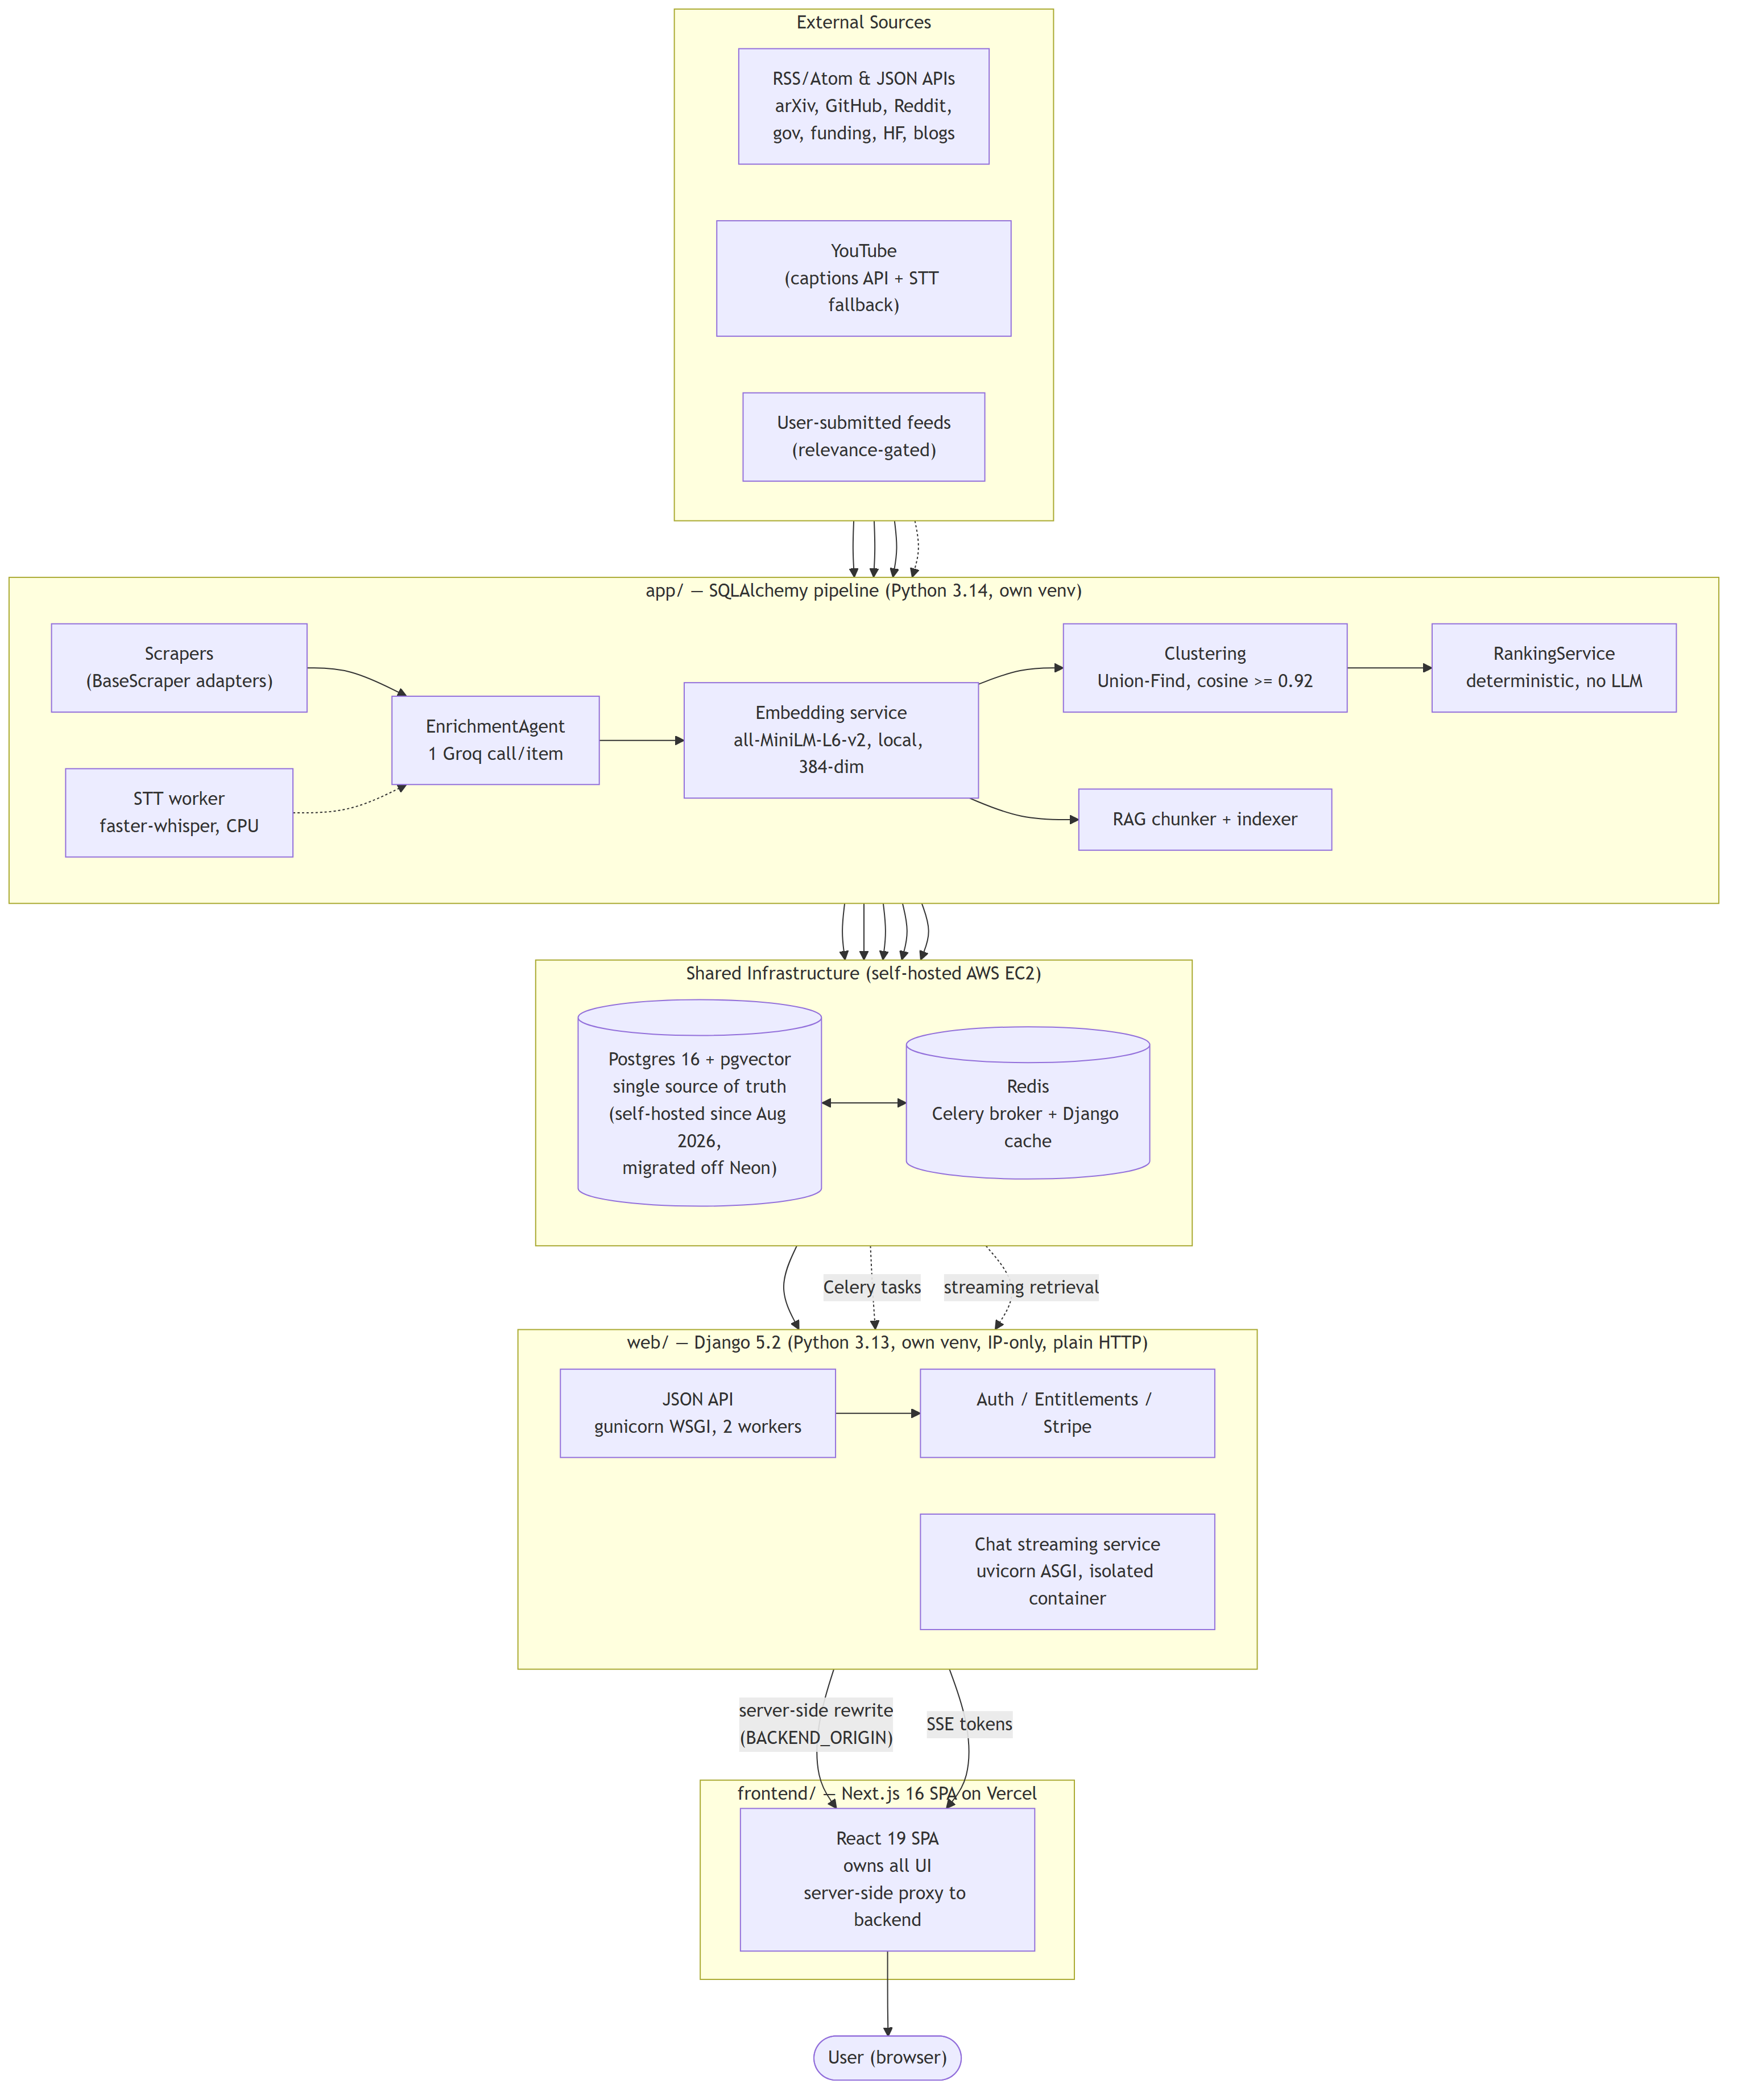
\includegraphics[width=0.85\textwidth,height=0.88\textheight,keepaspectratio]{figures/system_architecture.png}
\caption{AI Compass system architecture: external sources feed the
pipeline, which writes to a shared PostgreSQL+pgvector database; the Django
backend and Next.js frontend serve users, with a dedicated ASGI process
isolating the RAG assistant's SSE streaming from the main WSGI
application.}
\label{fig:sysarch}
\end{figure}

Figure~\ref{fig:sysarch} shows how these pieces fit together end to end. At
the top, \textbf{external sources} enter through three paths: RSS/Atom
feeds and JSON APIs (arXiv, GitHub, Reddit, government notices, funding
announcements, Hugging Face, and blogs), YouTube (captions API first,
speech-to-text fallback otherwise), and user-submitted feeds, gated by the
relevance check before their content is ever ingested. All three feed the
\textbf{pipeline}, whose five stages the figure exposes explicitly:
source-specific \textbf{scrapers} hand raw items to the
\textbf{EnrichmentAgent}, which makes the single structured LLM call per
item; its output is embedded by the local \textbf{embedding service};
embeddings feed both \textbf{clustering}, which groups near-duplicates, and
the \textbf{RAG chunker and indexer}, which builds the passage index the
assistant retrieves from; clustering output finally reaches the
deterministic \textbf{RankingService}. The dashed edge from the
\textbf{STT worker} into the EnrichmentAgent reflects that transcribed
video re-enters the same enrichment step as any other content, rather than
following a separate path.

Everything the pipeline produces is written to the \textbf{shared
infrastructure} box: a self-hosted PostgreSQL~16 instance with
\texttt{pgvector}, and Redis, both on the same AWS EC2 host. Redis serves a
dual role, drawn as one box connected bidirectionally to Postgres: it is
the Celery broker for the pipeline's background tasks and, separately, the
Django cache. From this shared store, the \textbf{Django backend} serves
two distinct kinds of traffic through two distinct processes: the
\textbf{JSON API}, under Gunicorn as a conventional WSGI application with
two synchronous workers, handling authentication, entitlements, Stripe, and
every ordinary request; and a \textbf{dedicated chat streaming service},
the same Django codebase's ASGI entry point under Uvicorn in its own
container. The two reach the shared infrastructure differently (the JSON
API dispatches Celery tasks and waits for a result, while the chat service
issues streaming retrieval calls), and the isolation exists specifically so
a long-lived server-sent-event connection can never occupy one of the JSON
API's only two workers. Finally, the \textbf{Next.js frontend}, on Vercel,
owns the entire UI and reaches the backend over two channels: a server-side
rewrite proxying ordinary API calls same-origin, and a direct SSE token
stream for chat, before rendering to the \textbf{user's browser}.

\section{Key Technology Decisions}
\label{sec:arch-tech-decisions}

Table~\ref{tab:techstack} summarizes the primary technology choices behind
each major layer of the system.

\begin{table}[htbp]
\centering
\caption{Key technology decisions across the three codebases.}
\label{tab:techstack}
\begin{tabular}{|p{3.8cm}|p{11cm}|}
\hline
\textbf{Layer} & \textbf{Choice} \\
\hline
Language / runtime & Python 3.14 (pipeline), Python 3.13 (Django), TypeScript / Next.js 16 (frontend) \\
\hline
Database & PostgreSQL 16 with the \texttt{pgvector} extension \\
\hline
Task queue & Celery with Redis as broker, split into \texttt{default}/\texttt{interactive}/\texttt{stt} queues \\
\hline
LLM provider & Groq (Llama~3.1~8B and Llama~3.3~70B tiers) \\
\hline
Embedding model & \texttt{all-MiniLM-L6-v2}, local, 384-dimensional \\
\hline
ASR & \texttt{faster-whisper} \texttt{distil-large-v3}, CPU-only \\
\hline
\end{tabular}
\end{table}

Each row in Table~\ref{tab:techstack} reflects a trade-off rather than a
default choice. The pipeline and the Django application sit on different,
independently upgradable Python versions because they are separate
deployment units with no shared runtime to reconcile, consistent with
Section~\ref{sec:arch-three-codebases}. PostgreSQL with \texttt{pgvector}
lets ordinary relational data and vector similarity search live in the one
database the cross-ORM boundary already depends on, rather than operating
a second, specialized vector store. Celery with Redis gives the system
three independently tunable queues: a slow speech-to-text job can never
delay the six-hourly batch pipeline, and neither can delay a live
user-facing search or assistant request, expanded on in
Section~\ref{sec:arch-task-orchestration}. Groq was chosen for its
low-latency inference of open-weight models, used at two tiers so
high-volume tasks (per-item enrichment, query condensation) run on the
smaller 8B model while assistant answer generation uses the larger 70B
model. \texttt{all-MiniLM-L6-v2} runs locally at negligible cost, avoiding
a per-call external dependency for an operation every ingested item and
every search query requires. \texttt{faster-whisper}'s
\texttt{distil-large-v3} was chosen as a CPU-only, no-GPU-required speech-
to-text engine, a constraint imposed by the project's deployment budget
rather than a performance-first choice; its measured throughput on that
hardware is reported in the evaluation chapter rather than assumed here.

\section{Background Task Orchestration}
\label{sec:arch-task-orchestration}

All scheduled and asynchronous work in AI Compass runs through Celery, with
work partitioned across three queues chosen to keep unrelated latency and
resource profiles from interfering with one another.

The \textbf{default} queue carries the pipeline's own scheduled work
(scraping, enrichment, embedding, clustering, and ranking) triggered on a
recurring six-hour cycle by Celery's beat scheduler rather than by any user
action. The \textbf{interactive} queue carries work a user is actively
waiting on: semantic search, retrieval for the conversational assistant,
and processing a newly submitted source, all of which need to feel like a
live, synchronous response and are therefore routed away from the default
queue so a long-running pipeline pass cannot delay them. The
\textbf{stt} queue isolates speech-to-text transcription because it is
CPU-heavy and can run for tens of minutes on a single long video; its own
queue and worker mean a transcription in progress never blocks the batch
pipeline or a live request on the interactive queue. This three-way
separation is a direct, mechanical consequence of the non-functional
requirements set out in Section~\ref{sec:req-nonfunctional}: an optional,
slow subsystem must be able to degrade in isolation without degrading the
rest of the system.
